\documentclass[10pt,a4paper,twocolumn]{report}
\usepackage[latin1]{inputenc}
\usepackage{amsmath}
\usepackage{amsfonts}
\usepackage{amssymb}
\usepackage{graphicx}
\usepackage{tikz}
\usepackage{tabularx}
\usepackage{lipsum}
\usetikzlibrary{matrix,calc}
\usepackage[margin=0.5in]{geometry}
\usepackage{tikz}
\usetikzlibrary{arrows,shapes.gates.logic.US,shapes.gates.logic.IEC,calc}
\usepackage{listings}

\begin{document}

\lstset{
frame=single, 
breaklines=true,
columns=fullflexible
}
\centering \textbf {\underline{ASSIGNMENT-1}}\\
\vspace{5mm}
\raggedright \textbf{Name} :\hspace{1mm} \textbf{Mannava Venkatasai} \\
\textbf{Roll}\hspace{3mm}   : \textbf{FWC22030} \\
\textbf{Email}\hspace{3mm} : \textbf{venkatasaimannava9948@gmail.com} \vspace{7mm} \\

\raggedright \textbf{PROBLEM STATEMENT:}\vspace{2mm}
\raggedright \\Draw the Logic Circuit for the following Boolean Expression :
\textbf{f(x,y,z,w) = ($x'$+y).z + $w'$}
\vspace{1cm}
\\ \textbf {Logic circuit:} \\
\vspace{10mm}
\tikzstyle{branch}=[fill,shape=circle,minimum size=1pt,inner sep=0pt]
\begin{tikzpicture}[label distance=1mm]

    \node (x3) at (0,0) {$x$};
    \node (x2) at (1,0) {$y$};
    \node (x1) at (2,0) {$z$};
    \node (x0) at (3,0) {$w$};

    \node[not gate US, draw, rotate=-90] at ($(x3)+(0,-1)$) (Not3) {};
    \node[not gate US, draw, rotate=-90] at ($(x0)+(0,-1)$) (Not0) {};

    \node[or gate US, draw, logic gate inputs=nn] at ($(x0)+(1,-2)$) (Or1) {};

    \node[and gate US, draw, logic gate inputs=nn, anchor=input 1] at ($(Or1.output)+(1,-1)$) (And1) {};
    \node[or gate US, draw, logic gate inputs=nn, anchor=input 1] at ($(Or1.output -| And1.output)+(1,-1.5)$) (Or2) {};

    \foreach \i in {3,0}
    {
        \path (x\i) -- coordinate (punt\i) (x\i |- Not\i.input);
        \draw (punt\i) node[branch] {} -| (Not\i.input);
    }
    \draw (x2) |- (Or1.input 2);
    \draw (Not3.output) |- (Or1.input 1);
    \draw (Or1.output) -- ([xshift=0.2cm]Or1.output) |- (And1.input 1);
    \draw (x1) |- (And1.input 2);
    \draw (And1.output) -- ([xshift=0.2cm]And1.output) |- (Or2.input 1);
    \draw (Not0.output) |- (Or2.input 2);
    \draw (Or2.output) -- ([xshift=0.5cm]Or2.output) node[above] {$f_1$};
   
    
  
\end{tikzpicture}
\vspace{5mm}
\\ \raggedright \textbf{\underline{AIM:}}\vspace{2mm}
\\ \raggedright To Draw the Logic Circuit and implement using vaman board for the following Boolean Expression :
\\ F(x,y,z,w) = ($x'$+y).z + $w'$
\vspace{5mm}
\\ \raggedright \textbf{\underline{Components:}}\vspace{2mm}
\begin{table}[ht]
\centering % used for centering table
\begin{tabular}{c c c} % centered columns (4 columns)
\hline\hline %inserts double horizontal lines
S.No & Component & Number \\ [0.5ex] % inserts table 
\hline
1 & Vamanboard & 1 \\
2 & Bread Board & 1 \\
3 & Jumer Wires(M-F) & 10 \\
4 & Seven segment display & 1 \\ [1ex] 
\hline
\end{tabular}
\end{table}
\vspace{5mm}
\\ \raggedright \textbf{\underline{Procedure:}}\vspace{4mm}
\begin{enumerate}
\item  Connect the seven segment display to the vaman board.
\item  Compile the source code in termux using make command.
\item bin files will be generated in the output folder 
\item Transfer the generated bin files to the laptop using scp command 
\item connect the vaman board to the laptop and flash the code in to the vaman board. 
\item The out put will be displayed in seven segment display either 1 or 0 corresponds to the out given boolean expression.
\end{enumerate}
\raggedright \textbf{\underline{OUTPUTS:}}\vspace{7mm}
\\ \raggedright \textbf{\underline{Truthtable:}}\vspace{2mm}
   \begin{center}
\begin{tabularx}{0.4\textwidth} { 
  | >{\centering\arraybackslash}X 
  | >{\centering\arraybackslash}X 
  | >{\centering\arraybackslash}X
  | >{\centering\arraybackslash}X
  | >{\centering\arraybackslash}X | }
\hline
\textbf{x} &\textbf{y} & \textbf{z} & \textbf{w} & \textbf{f} \\
\hline
0 & 0 & 0 & 0 & 1 \\  
\hline
0 & 0 & 0 & 1 & 0 \\ 
\hline
0 & 0 & 1 & 0 & 1 \\
\hline
0 & 0 & 1 & 1 & 1 \\
\hline
0 & 1 & 0 & 0 & 1 \\  
\hline
0 & 1 & 0 & 1 & 0 \\ 
\hline
0 & 1 & 1 & 0 & 1 \\
\hline
0 & 1 & 1 & 1  1 \\
\hline
1 & 0 & 0 & 0 & 1 \\
\hline
1 & 0 & 0 & 1 & 0 \\
\hline
1 & 0 & 1 & 0 & 1 \\
\hline
1 & 0 & 1 & 1 & 0 \\
\hline
1 & 1 & 0 & 0 & 1 \\
\hline
1 & 1 & 0 & 1 & 0 \\
\hline
1 & 1 & 1 & 0 & 1 \\
\hline
1 & 1 & 1 & 1 & 1 \\
\hline
\end{tabularx}
\end{center}
\raggedright \begin{center} 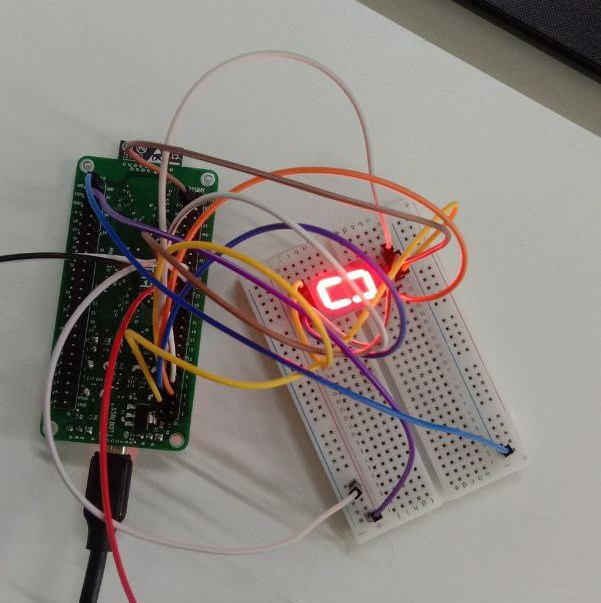
\includegraphics[scale=0.27]{arm0.jpeg} \end{center} \begin{center} The output is displayed as 0 in seven segment display corresponds to the given inputs. \end{center}
\vspace{5mm}
\raggedright \begin{center} 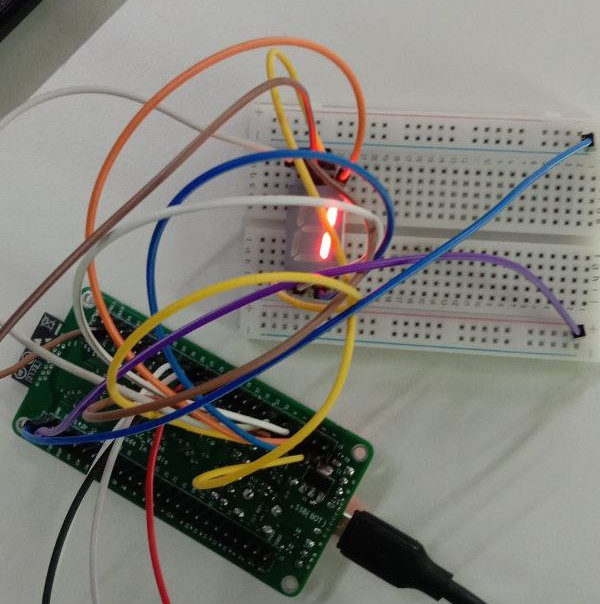
\includegraphics[scale=0.27]{arm1.jpeg} \end{center}
\begin{center} The output is displayed as 1 in seven segment display corresponds to the given inputs. \end{center}
\vspace{5mm}
\raggedright \textbf{\underline{Conclusion:}}\vspace{7mm}
\\ Hence I have drawn the logic circuit for the given logic expression and I have implemented the circuit in arduino and verified the outputs.
\end{document}&
